\documentclass[border=6pt]{standalone}
% Shared preamble for web figures.  Each figure is a standalone .tex that
% \input's this file; scripts/make-figures.sh turns it into an SVG.
% Handouts pull the same file with \fig{Unit_X/<name>}.
\usepackage[T1]{fontenc}
\usepackage{helvet}
\renewcommand{\familydefault}{\sfdefault}
\renewcommand{\ttdefault}{pcr}  % Courier: a real Type 1 typewriter font
\usepackage{amsmath}
\usepackage{tikz}
\usetikzlibrary{arrows.meta,positioning,calc,shapes.symbols,shapes.geometric}

% Who makes the rules is the point of most diagrams in this book, so the
% colors mean the same thing everywhere: blue is a person, orange is the
% computer, green is an answer, pink is the human brain.
\definecolor{person}{HTML}{2C6FAE}
\definecolor{machine}{HTML}{D35400}
\definecolor{result}{HTML}{1E8449}
\definecolor{brainpink}{HTML}{C2185B}
\definecolor{ink}{HTML}{2C3E50}

\tikzset{
  doodle/.style={line width=1.5pt, line cap=round, line join=round, draw=ink},
  box/.style={draw, rounded corners=5pt, line width=1.1pt, align=center,
              inner sep=7pt, minimum height=1.0cm, font=\small},
  personbox/.style={box, draw=person, fill=person!10},
  machinebox/.style={box, draw=machine, fill=machine!10},
  resultbox/.style={box, draw=result, fill=result!10},
  plainbox/.style={box, draw=ink!70, fill=ink!4},
  flow/.style={-{Stealth[length=8pt]}, line width=1.4pt, draw=ink},
}

% A person (blue) and a robot head (orange) as small icons.
% \personicon{x}{y}{scale}   \roboticon{x}{y}{scale}
\newcommand{\personicon}[3]{%
  \begin{scope}[shift={(#1,#2)}, scale=#3]
    \fill[person] (0,0.62) circle (0.28);
    \fill[person, rounded corners=6pt] (-0.42,-0.55) rectangle (0.42,0.28);
  \end{scope}}
\newcommand{\roboticon}[3]{%
  \begin{scope}[shift={(#1,#2)}, scale=#3]
    \draw[machine, line width=1.2pt] (0,0.5) -- (0,0.72);
    \fill[machine] (0,0.78) circle (0.08);
    \draw[machine, line width=1.4pt, fill=machine!12, rounded corners=4pt] (-0.5,-0.45) rectangle (0.5,0.5);
    \fill[ink] (-0.2,0.12) circle (0.08);
    \fill[ink] (0.2,0.12) circle (0.08);
    \draw[ink, line width=1pt] (-0.22,-0.22) -- (0.22,-0.22);
  \end{scope}}

\begin{document}
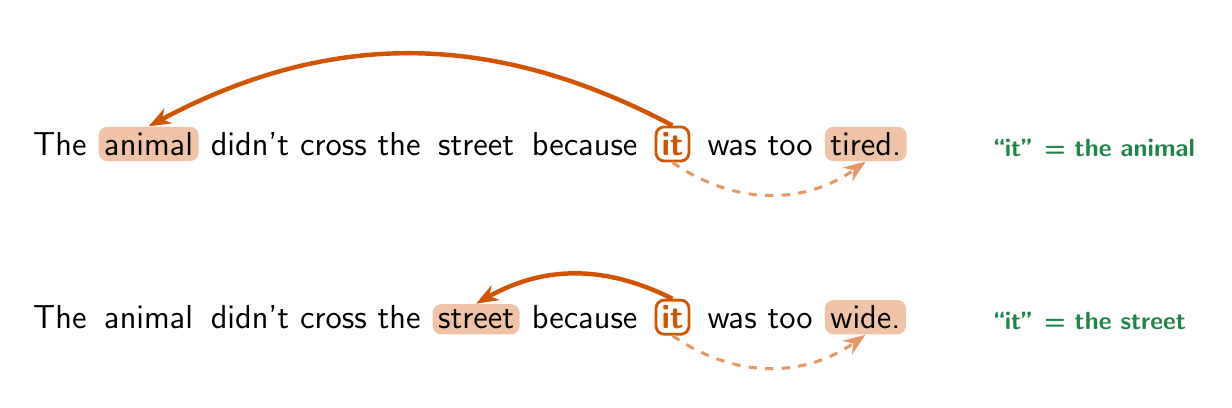
\begin{tikzpicture}[
  w/.style={inner sep=2pt, font=\large, anchor=base},
  hot/.style={w, fill=machine!35, rounded corners=3pt},
  it/.style={w, text=machine, font=\large\bfseries, draw=machine, rounded corners=3pt, line width=1pt},
]
% "it" looks back at the other words; the last word decides which noun.
\newcommand{\sentence}[5]{% #1 row name, #2 y, #3 style of animal, #4 style of street, #5 last word
  \node[w] (a#1) at (0,#2) {The};
  \node[#3, right=2pt of a#1.base east, anchor=base west] (b#1) {animal};
  \node[w, right=2pt of b#1.base east, anchor=base west] (c#1) {didn't cross the};
  \node[#4, right=2pt of c#1.base east, anchor=base west] (d#1) {street};
  \node[w, right=2pt of d#1.base east, anchor=base west] (e#1) {because};
  \node[it, right=4pt of e#1.base east, anchor=base west] (f#1) {it};
  \node[w, right=4pt of f#1.base east, anchor=base west] (g#1) {was too};
  \node[hot, right=2pt of g#1.base east, anchor=base west] (h#1) {#5.};}
\sentence{1}{0}{hot}{w}{tired}
\sentence{2}{-2.2}{w}{hot}{wide}
\draw[flow, draw=machine, line width=1.6pt] (f1.north) to[bend right=28] (b1.north);
\draw[flow, draw=machine, line width=1.6pt] (f2.north) to[bend right=28] (d2.north);
\draw[flow, draw=machine!60, line width=1.1pt, dashed] (f1.south) to[bend right=35] (h1.south);
\draw[flow, draw=machine!60, line width=1.1pt, dashed] (f2.south) to[bend right=35] (h2.south);
\node[anchor=west, font=\small\bfseries, text=result] at (11.7,0.1) {``it'' = the animal};
\node[anchor=west, font=\small\bfseries, text=result] at (11.7,-2.1) {``it'' = the street};
\end{tikzpicture}
\end{document}
